\section{Corrections and systematic uncertainties for simulation}
\label{sec:htoinv_mc_corrections}

In order for simulated events, particularly \acrshort{sm} background processes, to resemble \acrshort{lhc} data as closely as possible, many corrections are applied. These are discussed in more detail in the subsequent sections. All corrections and associated systematic uncertainties are applied to all samples for all data taking years, unless stated otherwise, and summarised in Tab.~\ref{tab:htoinv_syst_summary}.

A final event weight $w_{\mathrm{event}}$ is the product of the weights from all of the individual sources $i$ that provide one:
\begin{equation}
    w_{\mathrm{event}} = \prod_i w_i.
    \label{eq:event_weight}
\end{equation}
When representing these events in histograms, the yield in a given bin $N_{\mathrm{corr.}}$ is the sum of these event weights:
\begin{equation}
    N_{\mathrm{corr.}} = \sum_j^{N_{\mathrm{MC}}} w_{\mathrm{event} \ j},
    \label{eq:bin_weight}
\end{equation}
where $N_{\mathrm{MC}}$ is the number of unweighted, simulated events in the bin. In the data--\acrshort{mc} distributions shown previously in this chapter, the statistical uncertainty ascribed to the \acrshort{mc} yield in a bin is estimated from the unweighted number of events ($k$ in a Poisson statistical treatment):
\begin{equation}
    \Delta N_{\mathrm{corr.}} = \pm \frac{ N_{\mathrm{corr.}} }{ \sqrt{N_{\mathrm{MC}}} }.
    \label{eq:uncertainty_mc_ours}
\end{equation}
While the statistical uncertainty for the number of events in data is simply the Poissonian error,
\begin{equation}
    \Delta N_{\mathrm{data}} = \pm \frac{ N_{\mathrm{data}} }{ \sqrt{N_{\mathrm{data}}} }.
    \label{eq:uncertainty_data}
\end{equation}


%=========================================================


\subsection{Efficiency of the triggers}
\label{subsec:htoinv_trigger_effs}

Given the modelling of the \acrlong{l1} and \acrlong{hlt} systems in simulation is only an approximation of their behaviour with real data, corrections must be applied to ensure it is more representative of the data collected by \acrshort{cms}.

A dedicated \gls{CR} is formed to assure orthogonality with the signal region and avoid unblinding of data, but with a similar kinematic selection to the analysis for accuracy in the desired phase space. Events are selected in data from the primary dataset consisting of muon-based triggers, and in simulation from the \wtolnupjets process at \acrshort{lo}. Analysed events contain a single, tightly-isolated muon with $\pt > \text{30}\GeV$ that triggers the \acrshort{hlt} path for an isolated muon with $\pt > \text{27}\GeV$. This is to avoid biasing the efficiencies of the triggers defining the signal region. An offline selection is then applied to keep those with similar kinematic properties to those in the signal region:

\medskip
\begin{easylist}[itemize]
    \cutflowlistprops
    & $\ptjone > \text{80}\GeV$
    & $\HT > \text{200}\GeV$
    & $\mht/\ptmissNoMu < \text{1.2}$
\end{easylist}

\medskip

\noindent{}where $\ptmissNoMu = \lvert \ptvecmiss + \ptvec^{\kern1pt \Pmu} \rvert$ to approximate the \acrshort{pf} calculation at \acrshort{hlt} level. Of these, events that additionally pass the online selection of the trigger requirements in the signal region (Tab.~\ref{tab:htoinv_SR_triggers}) are also recorded. The efficiency of a trigger---or collection of triggers---$\epsilon_{\mathrm{trg}}$ is defined as
\begin{equation}
    \epsilon_{\mathrm{trg}} = \frac{ s_\mathrm{offline} \cap s_{\mathrm{online}} }{ s_\mathrm{offline} },
    \label{eq:trigger_eff}
\end{equation}
where $s$ denotes the set of events that have passed the selection given by its subscript. For simulation, events are weighted by cross section as per Eq.~\ref{eq:xs_weight}. The efficiencies are binned in two dimensions as a function of \ptmissNoMu and \mht. The weight applied to events in simulation $w_{\mathrm{trg}}$ is then simply the efficiency in data divided by the efficiency in simulation for the values of \ptmiss and \mht in the event:
\begin{equation}
    w_{\mathrm{trg}}(\ptmiss, \mht) = \frac{\epsilon_{\mathrm{trg, \ data}}(\ptmiss, \mht)}{\epsilon_{\mathrm{trg, \ MC}}(\ptmiss, \mht)}.
    \label{eq:trigger_weight}
\end{equation}
Uncertainties are estimated using the Clopper-Pearson method~\cite{10.1093/biomet/26.4.404} and impact the yields by up to 1--2\,\%. In the signal region, sidebands, and muon \glspl{CR}, weights from the efficiencies of the \ptmiss--\mht cross triggers are used. The weights are provided for each data taking year in Fig.~\ref{fig:htoinv_trig_effs}. In the electron and photon \glspl{CR}, the efficiencies are calculated in the same manner, instead with the triggers in Tabs.~\ref{tab:htoinv_ele_pd_triggers} and \ref{tab:htoinv_photon_pd_triggers}.

\clearpage

\begin{figure}[htbp]
    \centering
    \begin{subfigure}[b]{0.49\textwidth}
        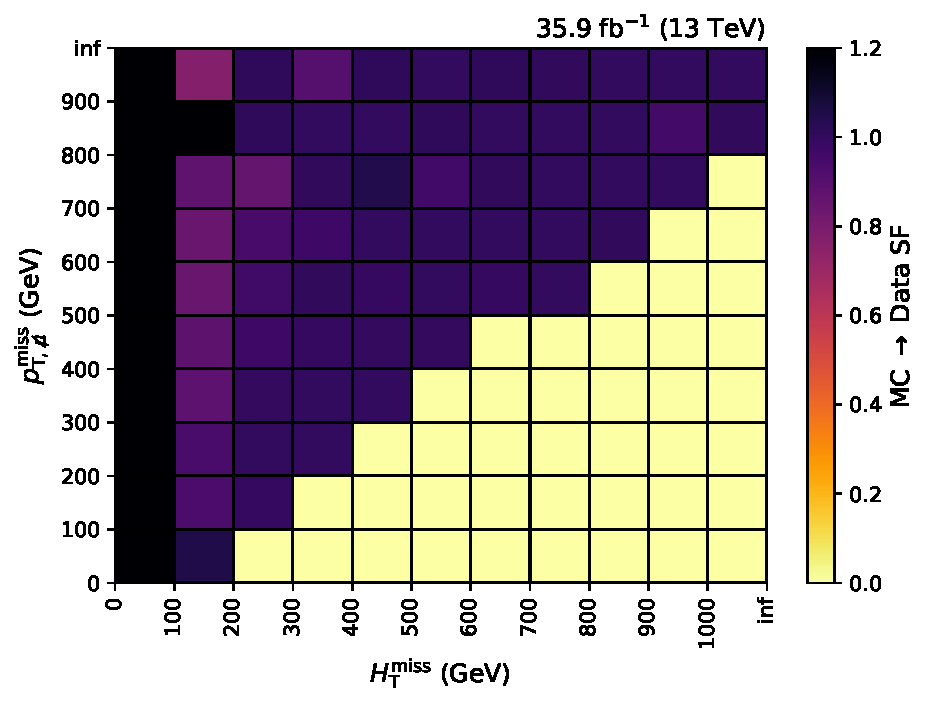
\includegraphics[width=\textwidth]{figures/trigger_efficiencies/2016/SFs.pdf}
        \caption{2016}
    \end{subfigure}
    \hfill
    \begin{subfigure}[b]{0.49\textwidth}
        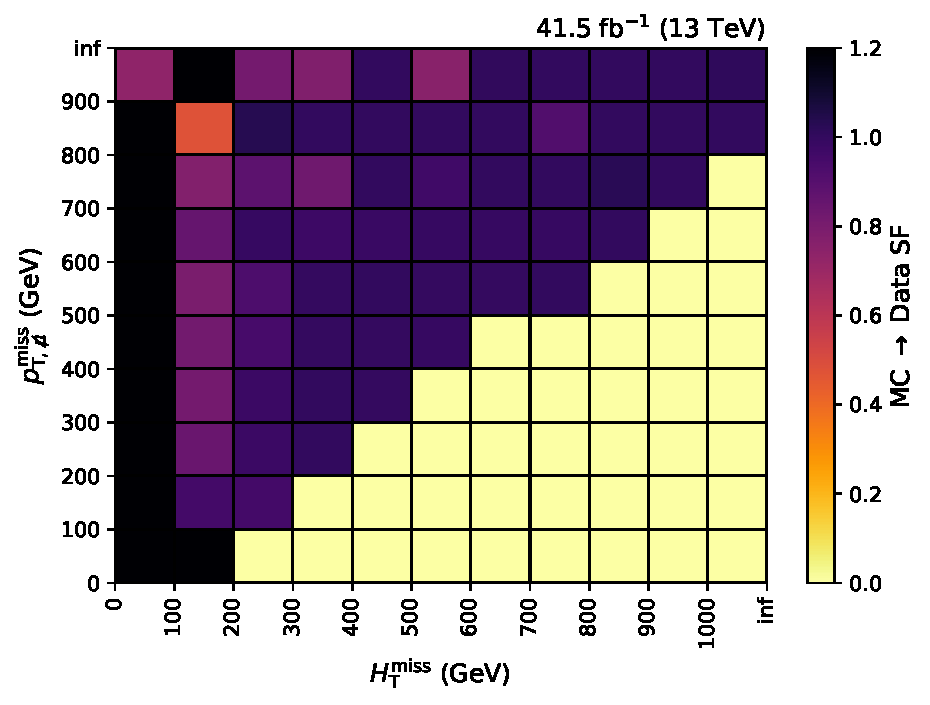
\includegraphics[width=\textwidth]{figures/trigger_efficiencies/2017/SFs.pdf}
        \caption{2017}
    \end{subfigure}

    \begin{subfigure}[b]{0.49\textwidth}
        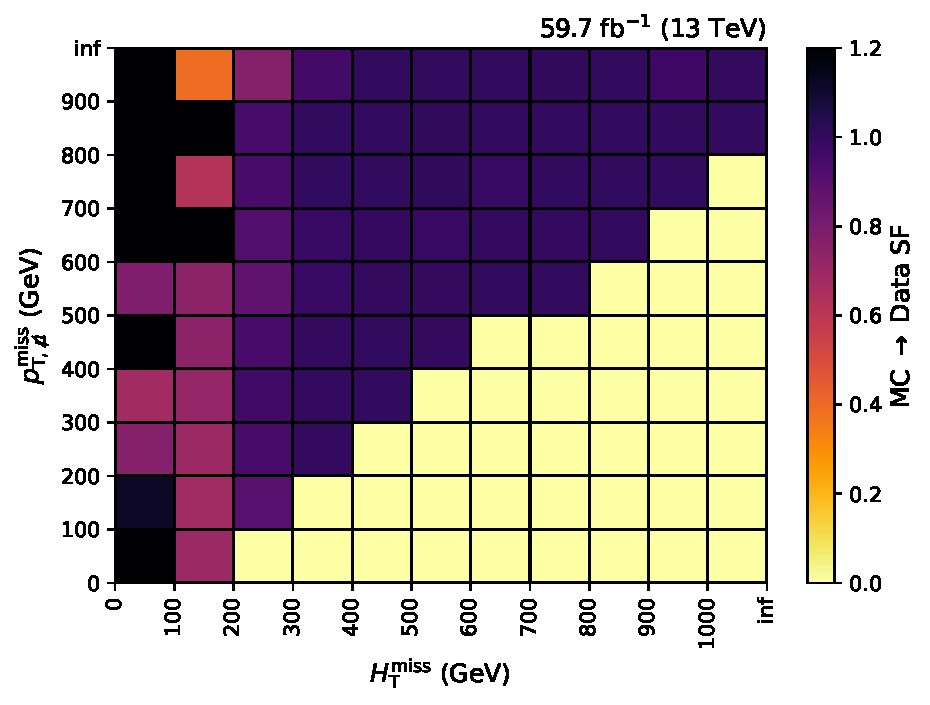
\includegraphics[width=\textwidth]{figures/trigger_efficiencies/2018/SFs.pdf}
        \caption{2018}
    \end{subfigure}
    \caption[Scale factors accounting for the efficiencies of the HLT \ptmiss--\mht cross triggers in each data taking year of Run-2]{Scale factors accounting for the efficiencies of the \acrshort{hlt} \ptmiss--\mht cross triggers in each data taking year of Run-2. The momentum of the muon used to select events that compute the efficiency is added to the \ptvecmiss (with a magnitude \ptmissNoMu) in order to approximate the calculation in the \acrlong{hlt}.}
    \label{fig:htoinv_trig_effs}
\end{figure}


%=========================================================


\subsection{Pileup reweighting}
\label{subsec:pu_reweighting}

\Gls{pileup} interactions at the \acrshort{lhc} are frequent (see Sec.~\ref{subsec:pileup}) and must be modelled appropriately in simulation. Simulated samples are generated with a certain distribution of the number of \gls{pileup} interactions which usually does not match the data recorded by \acrshort{cms}. This is due to changing conditions in the beam over a period of data taking. In order to make them comparable, the simulated events are reweighted; in this context it is known as \emph{\gls{pileup} reweighting}. \ROOT files containing histograms of the number of \gls{pileup} interactions from short runs in the \acrshort{lhc} are available centrally and are used as the reference for which to reweight the simulated events.

Simulated events are nominally reweighted according to data, where the inelastic $\pp$ cross section is measured to be 69.2\,mb. An uncertainty of $\pm \text{4.6}$\,\% in the measurement is used to calculate the systematic uncertainty on this weight. These were found to be a 1--2\,\% effect in the signal and \glspl{CR}. The pileup distributions, and therefore the weights, are different for each data taking year. However, the inelastic cross section and associated uncertainty are consistent for the entirety of Run-2.

% https://github.com/cms-nanoAOD/nanoAOD-tools/blob/048a828e1d7f5ac3346e2f5e7eafba2570e84bc4/python/postprocessing/modules/common/puWeightProducer.py for implementation


%=========================================================


\subsection{Higher order corrections to \texorpdfstring{$\PVec \plusjets$}{V plus jets} samples}
\label{subsec:htoinv_nlo_corrs}

Vector boson $+$ \glspl{jet} processes present a sizeable background in the signal region for some of the categories, and are a large component of some of the \glspl{CR}. At the dataset sizes required to provide sufficient statistical coverage of the analysis phase space, \acrshort{nlo} \acrshort{mc} samples are not available with the complete detector simulation applied. To circumvent this, \acrshort{lo} samples are used primarily and reweighted at generator level on an event-by-event basis to \acrshort{nlo} accuracy. This method is usually referred to as a ``$k$-factor'' correction, where $k$ is the ratio of the \acrshort{nlo} to \acrshort{lo} cross section.

Separate \acrshort{nlo} \acrshort{qcd} and electroweak corrections are applied to the \acrshort{qcd} production of $\PVec \plusjets$ samples. \acrshort{nlo} $\PW \plusjets$ samples are utilised when deriving the $k$-factors for the \acrshort{lo} counterpart. Drell-Yan $\HepProcess{\PZ (\to \Plepton\APlepton)} \plusjets$ samples are utilised for both the \acrshort{lo} Drell-Yan and \ztonunupjets processes. The $k$-factors are calculated independently for the two processes as the \acrshort{lo} sample production and cross sections are different. One or two additional \glspl{jet} in the matrix element calculations are permitted in the \acrshort{nlo} samples. Events from the above datasets are processed through the following generator-level event selection to ensure they are in a similar phase space to the analysis:

\medskip
\begin{easylist}[itemize]
    \cutflowlistprops
    & $\ptjone > \text{80}\GeV$
    & $\pt^{\PVec} > \text{200}\GeV$
    & $\HT^{\mathrm{Gen}} > \text{200}\GeV$
    & $\HT^{\mathrm{Gen}}/\pt^{\PVec} < \text{1.2}$
\end{easylist}

\medskip

\noindent{}where $\pt^{\PVec}$ is the generator-level boson \pt, and $\HT^{\mathrm{Gen}}$ is the scalar sum of generator-level \gls{jet} \pt. The $k$-factors are binned in two dimensions, $\pt^{\PVec}$ and $\ptjone$.

Uncertainties for the \acrshort{qcd} renormalisation scale, factorisation scale, and in the parton distribution function are treated as individual, uncorrelated sources. The same values for the nominal $k$-factors and uncertainties are used for each data taking year in Run-2. The impact of the renormalisation scale uncertainty was approximately 0--5\,\% on the yields, while the factorisation and \acrshort{pdf} scales had effects of roughly 1--10\,\% and 1--5\,\%, respectively. Distributions of the \acrshort{nlo} \acrshort{qcd} $k$-factors are presented in Fig.~\ref{fig:htoinv_nlo_k_factors_qcd}.

\begin{figure}[htbp]
    \centering
    \begin{subfigure}[b]{0.49\textwidth}
        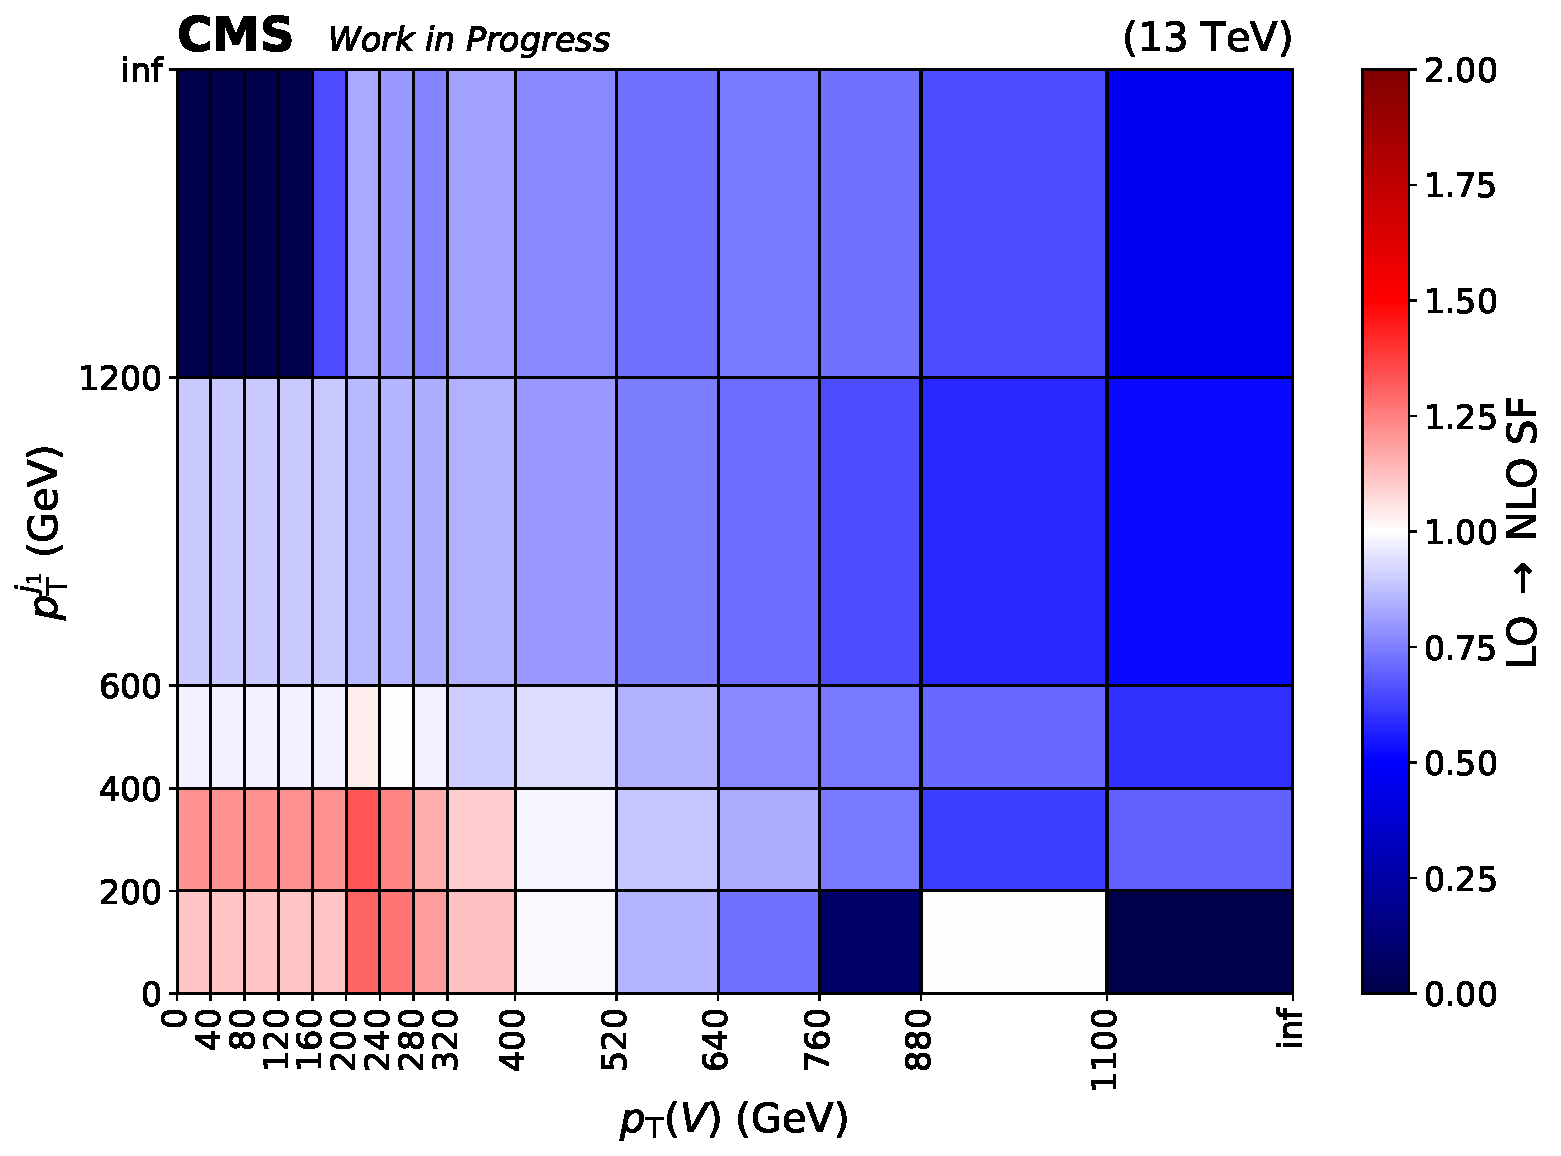
\includegraphics[width=\textwidth]{figures/nlo_k_factors/2D_zll.pdf}
        \caption{Drell-Yan $\HepProcess{\PZ \to \Plepton\APlepton}\plusjets$}
    \end{subfigure}
    \hfill
    \begin{subfigure}[b]{0.49\textwidth}
        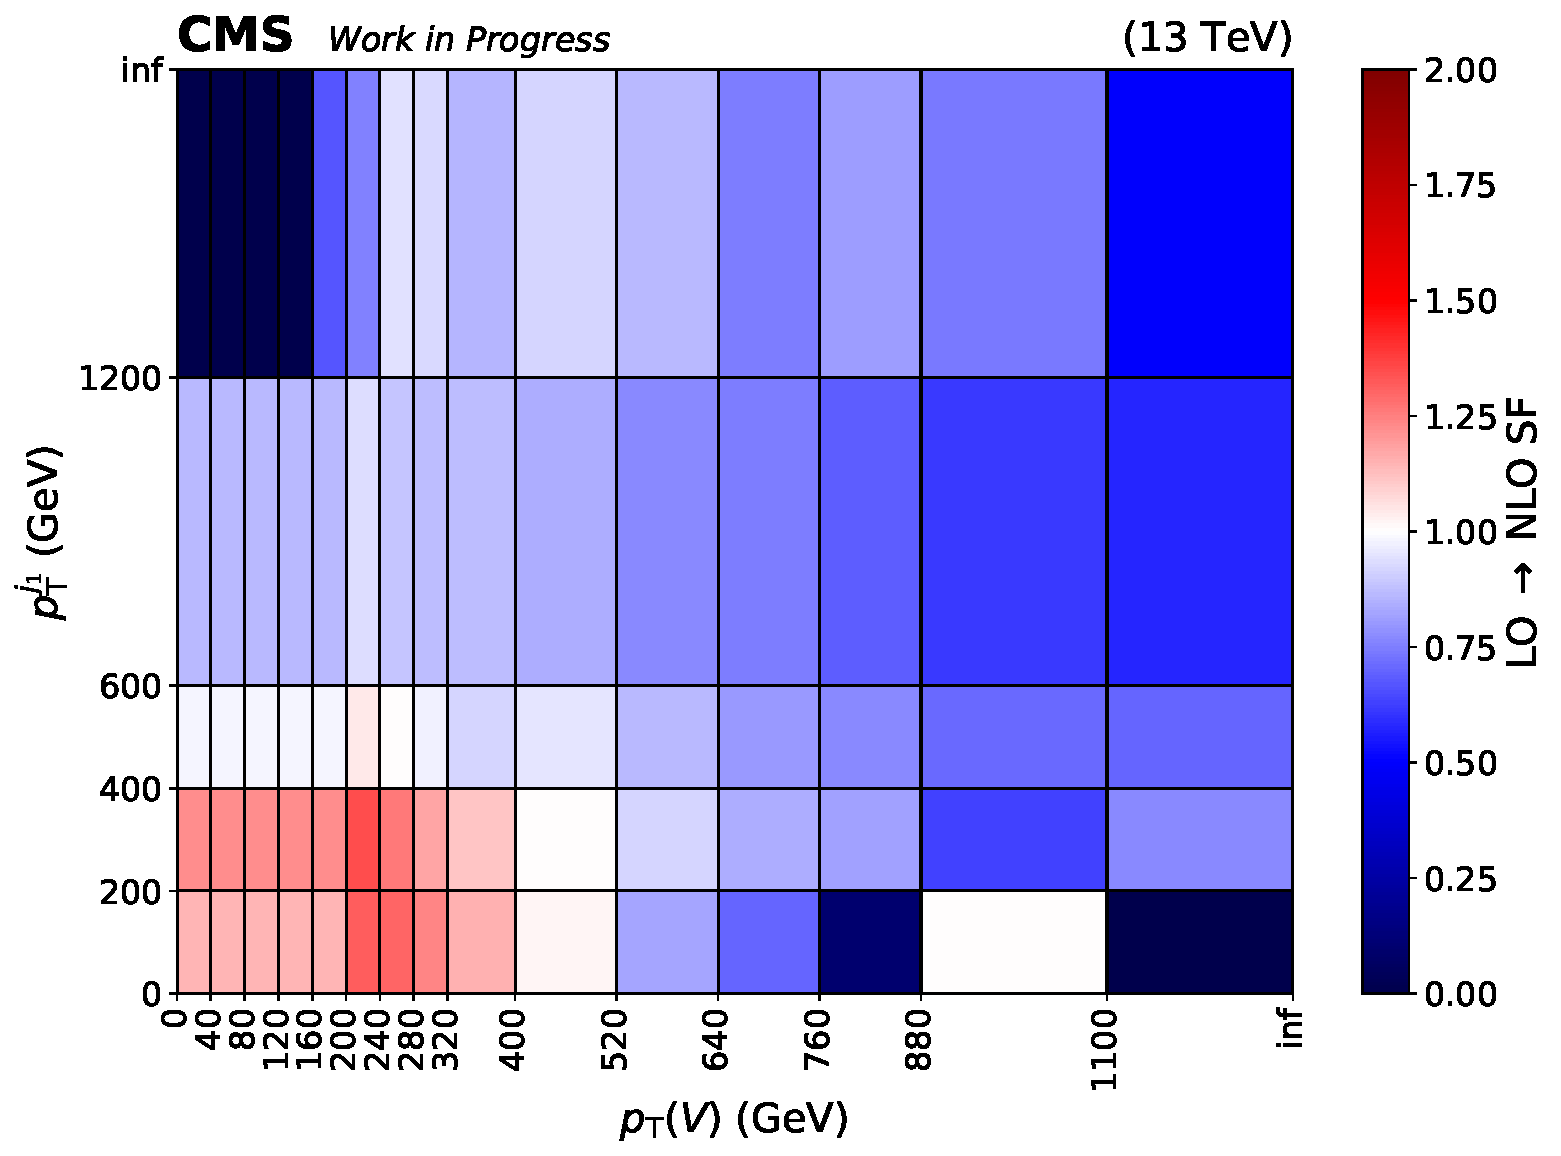
\includegraphics[width=\textwidth]{figures/nlo_k_factors/2D_znunu.pdf}
        \caption{$\ztonunupjets$}
    \end{subfigure}

    \begin{subfigure}[b]{0.49\textwidth}
        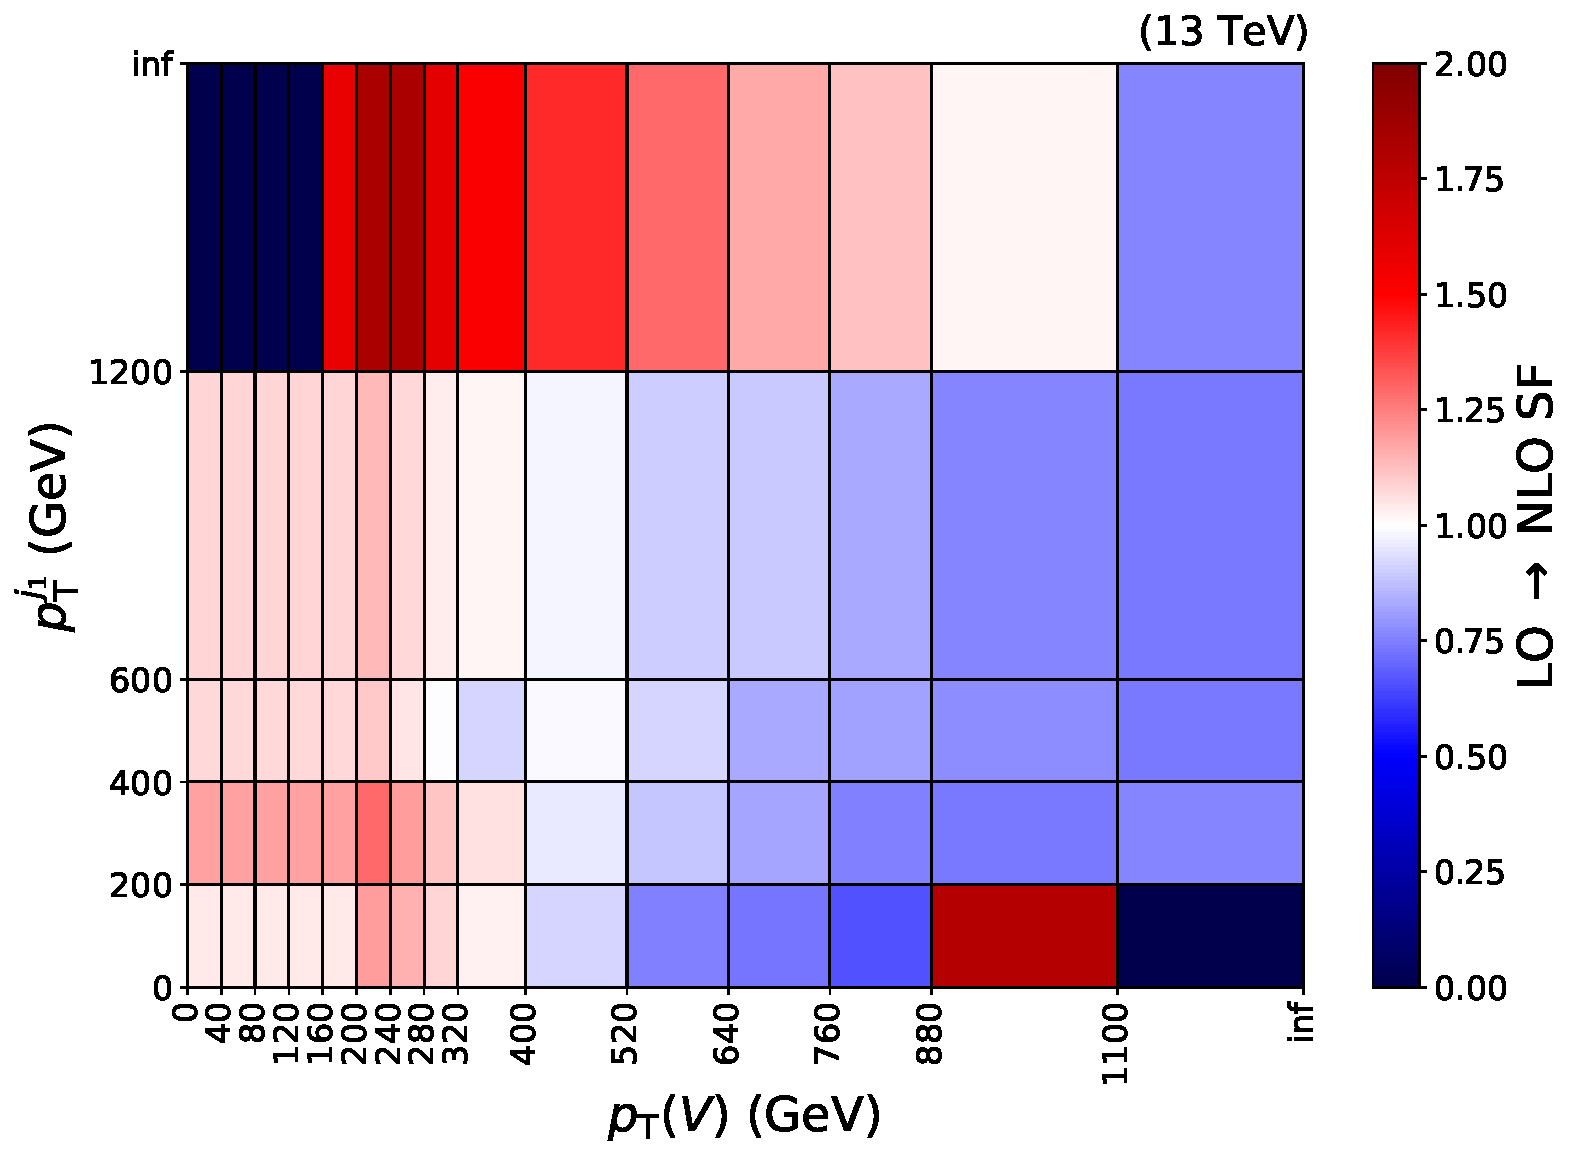
\includegraphics[width=\textwidth]{figures/nlo_k_factors/2D_wjets.pdf}
        \caption{$\wtolnupjets$}
    \end{subfigure}
    \caption[NLO $k$-factors---as a function of the generator-level boson \pt and leading jet \pt---for reweighting events in LO QCD $\PW$ and $\PZ \plusjets$ simulation to NLO accuracy in QCD]{\acrshort{nlo} $k$-factors---as a function of the generator-level boson \pt and leading jet \pt---for reweighting reweight events in \acrshort{lo} \acrshort{qcd} $\PW$ and $\PZ \plusjets$ simulation to \acrshort{nlo} accuracy in \acrshort{qcd}.}
    \label{fig:htoinv_nlo_k_factors_qcd}
\end{figure}

Since all of the $\PVec \plusjets$ samples were generated at \acrshort{lo} electroweak accuracy, an additional $k$-factor is needed to reweight events to \acrshort{nlo}. Ref.~\citenum{Lindert_2017}{}provides \acrshort{nlo} electroweak corrections for \PW, \PZ, and $\Pphoton\plusjets$ processes as a function of $\pt^{\PVec}$, depicted in Fig.~\ref{fig:htoinv_nlo_k_factor_ewk}. The \PZ $k$-factor is adopted by both the Drell-Yan and \ztonunu processes.

\clearpage

\begin{figure}[htbp]
    \centering
    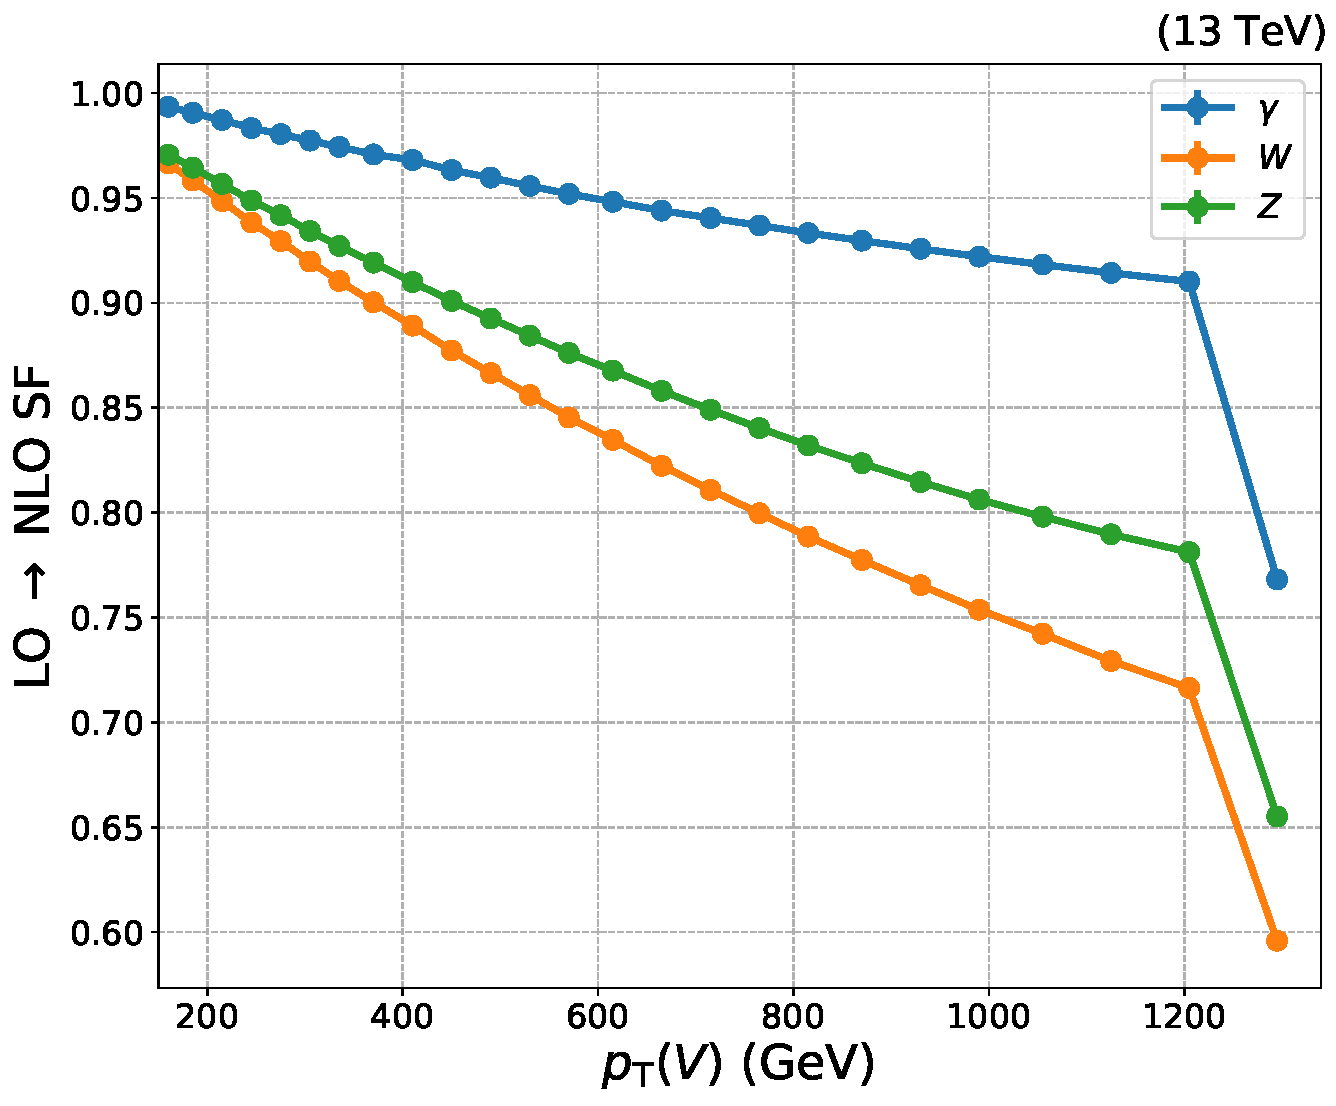
\includegraphics[width=0.52\textwidth]{figures/nlo_k_factors/1D_all_ewk.pdf}
    \caption[NLO $k$-factors as a function of generator-level boson \pt for reweighting QCD $\PVec \plusjets$ events generated at LO electroweak accuracy]{\acrshort{nlo} $k$-factors as a function of generator-level boson \pt for reweighting \acrshort{qcd} $\PVec \plusjets$ events generated at \acrshort{nlo} electroweak accuracy. Separate $k$-factors correct the \PW, \PZ, and $\Pphoton\plusjets$ processes. Values obtained from Ref.~\citenum{Lindert_2017}.}
    \label{fig:htoinv_nlo_k_factor_ewk}
\end{figure}


%=========================================================


\subsection{Top quark processes}
\label{subsec:htoinv_ttbar_uncerts}

\ttbarpjets is the dominant background for the \ttH channel. The $\ttbar X$ backgrounds also have a non-negligible presence. As such, much effort must be made to ensure they are modelled correctly. Variations of the \acrshort{qcd} renormalisation and factorisation scales provide an uncertainty only to the shape of the \ptmiss spectrum of the \ttbar and $\ttbar X$ backgrounds, and \ttH signal. Reweighting of the top quark \pt distribution to \acrshort{nnlo} accuracy is also performed for \ttbar, yielding a shape correction and associated uncertainty.


%=========================================================


\subsubsection{QCD scale systematic uncertainty}
\label{subsubsec:ttbar_renorm_fact_scale_uncert}

The renormalisation \muR and factorisation scale \muF chosen for \acrshort{mc} samples at generation may be somewhat arbitrary, and therefore not representative of nature. Relative to the nominal value, weights were derived centrally for each combination of these scales being varied independently (and together) up or down by a factor of two. Eight variations then exist for each event:
\medskip
\begin{easylist}[itemize]
    \easylistprops
    & $\muRAmuFB{\downarrow}{\downarrow}$
    & $\muRAmuFB{\downarrow}{\, \mathrm{nom.}}$
    & $\muRAmuFB{\downarrow}{ \uparrow}$
    & $\muRAmuFB{\, \mathrm{nom.}}{\downarrow}$
    & $\muRAmuFB{\, \mathrm{nom.}}{ \uparrow}$
    & $\muRAmuFB{\uparrow}{\downarrow}$
    & $\muRAmuFB{\uparrow}{\, \mathrm{nom.}}$
    & $\muRAmuFB{\uparrow}{\uparrow}$
\end{easylist}

\medskip

\noindent{}To remove the dependence on normalisation (since the skim and event selection may bias it) and ensure the systematic is only shape-based, each variation was also multiplied by an additional factor $f_{\mathrm{var}}$:
\begin{equation}
    f_{\mathrm{var}} = \dfrac{ \sum_{\text{unskimmed events}} w_{\mu_{\mathrm{R \, nom.}}\, \& \, \mu_{\mathrm{F \, nom.}} } }{ \sum_{\text{unskimmed events}} w_{\mathrm{var}} }.
    \label{eq:ttbar_scale_fvar}
\end{equation}
These are computed individually for each decay and data taking year. The envelope is characterised by the correlated variations $\muRAmuFB{\uparrow}{\uparrow}$, and $\muRAmuFB{\downarrow}{\downarrow}$. Confirmed by Fig.~\ref{fig:htoinv_ttbar_scale}, an example is given for the \ttbar background in the signal region. While the sizes of the variations appear large, they are reduced when matching the fit binning, and very similar between the signal and \glspl{CR}, cancelling to a large degree to minimally impact the results.

\begin{figure}[htbp]
    \centering
    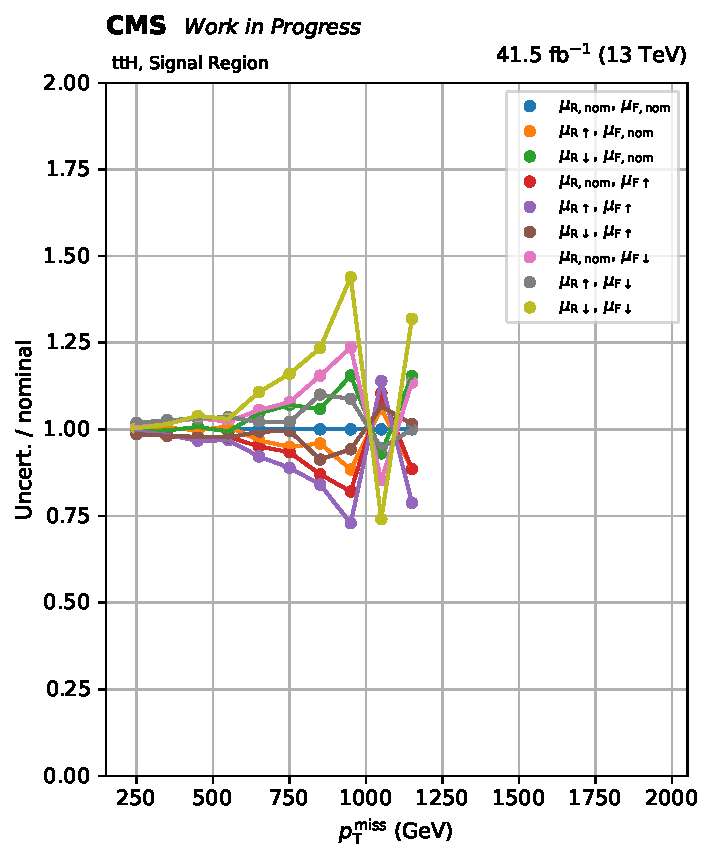
\includegraphics[width=0.5\textwidth]{figures/qcd_scale_top_procs/ttbar/ratio_vars_SR_ttH.pdf}
    \caption[The deviations relative to the nominal weight of the combinations of QCD renormalisation and factorisation scale variations. They are presented as a function of \ptmiss inclusive over the \ttH categories for the \ttbar samples]{The deviations relative to the nominal weight of the combinations of \acrshort{qcd} renormalisation and factorisation scale variations. They are presented as a function of \ptmiss inclusive over the \ttH categories for the \ttbar samples. Events are from the signal region in the 2017 dataset after the analysis-level selection.}
    \label{fig:htoinv_ttbar_scale}
\end{figure}

For each process (i.e., \ttbar, and the accompanying boson $X$ in $\ttbar X$), a separate systematic uncertainty is derived.\footnote{$\ttH(\HepProcess{\PH \to \text{invisible}})$ signal and $\ttH(\HepProcess{\PH \to \text{visible}})$ background are grouped as one process since the kinematics and generation procedure are consistent.} Since different generators and settings may be used for each dataset, it is appropriate to assume they are uncorrelated.


%=========================================================


\subsubsection{Top quark \texorpdfstring{\pt}{pT} reweighting}
\label{subsubsec:htoinv_top_pt_reweighting}

The top quark \pt distribution has been shown to be harder in simulation at \acrshort{nlo} than in data~\cite{Sirunyan:2018ucr}. \acrshort{nlo} \ttbarpjets \acrshort{mc} generated in \POWHEG is reweighted to \acrshort{nnlo} \acrshort{qcd} $+$ \acrshort{nlo} electroweak accuracy as function of top quark \pt. An analytic function fits the distribution that determines the weight. The same nominal function applies to all \ttbarpjets samples for all data taking years:
\begin{equation}
    f(\pt) = \exp(a + b \cdot \pt + c \cdot \pt^2),
\end{equation}
where the coefficients are $a = \text{1.614} \times \text{10}^{-2}$, $b = -\text{1.966} \times \text{10}^{-4}$, and $c = -\text{1.454} \times \text{10}^{-8}$. For a top or antitop quark, the scale factor is given by the value of $f$ for the particle's generator-level \pt. The event weight is then the square root of the product of the top and antitop scale factors.

The uncertainties are acquired from the fit itself over the theoretical uncertainties inherent in \acrshort{mc} calculations. This was to avoid double counting with respect to the renormalisation and factorisation scale uncertainty in Sec.~\ref{subsubsec:ttbar_renorm_fact_scale_uncert}, as overlap would be present and otherwise difficult to disentangle. For each parameter in the fit, the upward and downward variations were estimated. The fit function was then recalculated, fixing the parameter of interest to the variation. Providing upward and downward functions, the systematic uncertainty attributed to the parameter is simply the event weight calculated with these functions over the nominal. Separate, uncorrelated uncertainties were estimated for each parameter in the fit, and were each found to have a $< \text{2\,\%}$ impact on the event yields. The dependence on normalisation was removed in the same fashion as for the \acrshort{qcd} scale to consider the correction only to the shape of the distributions and not also the normalisation. The nominal function and associated variations are shown in Fig.~\ref{fig:top_pt_reweighting}.

\clearpage

\begin{figure}[htbp]
    \centering
    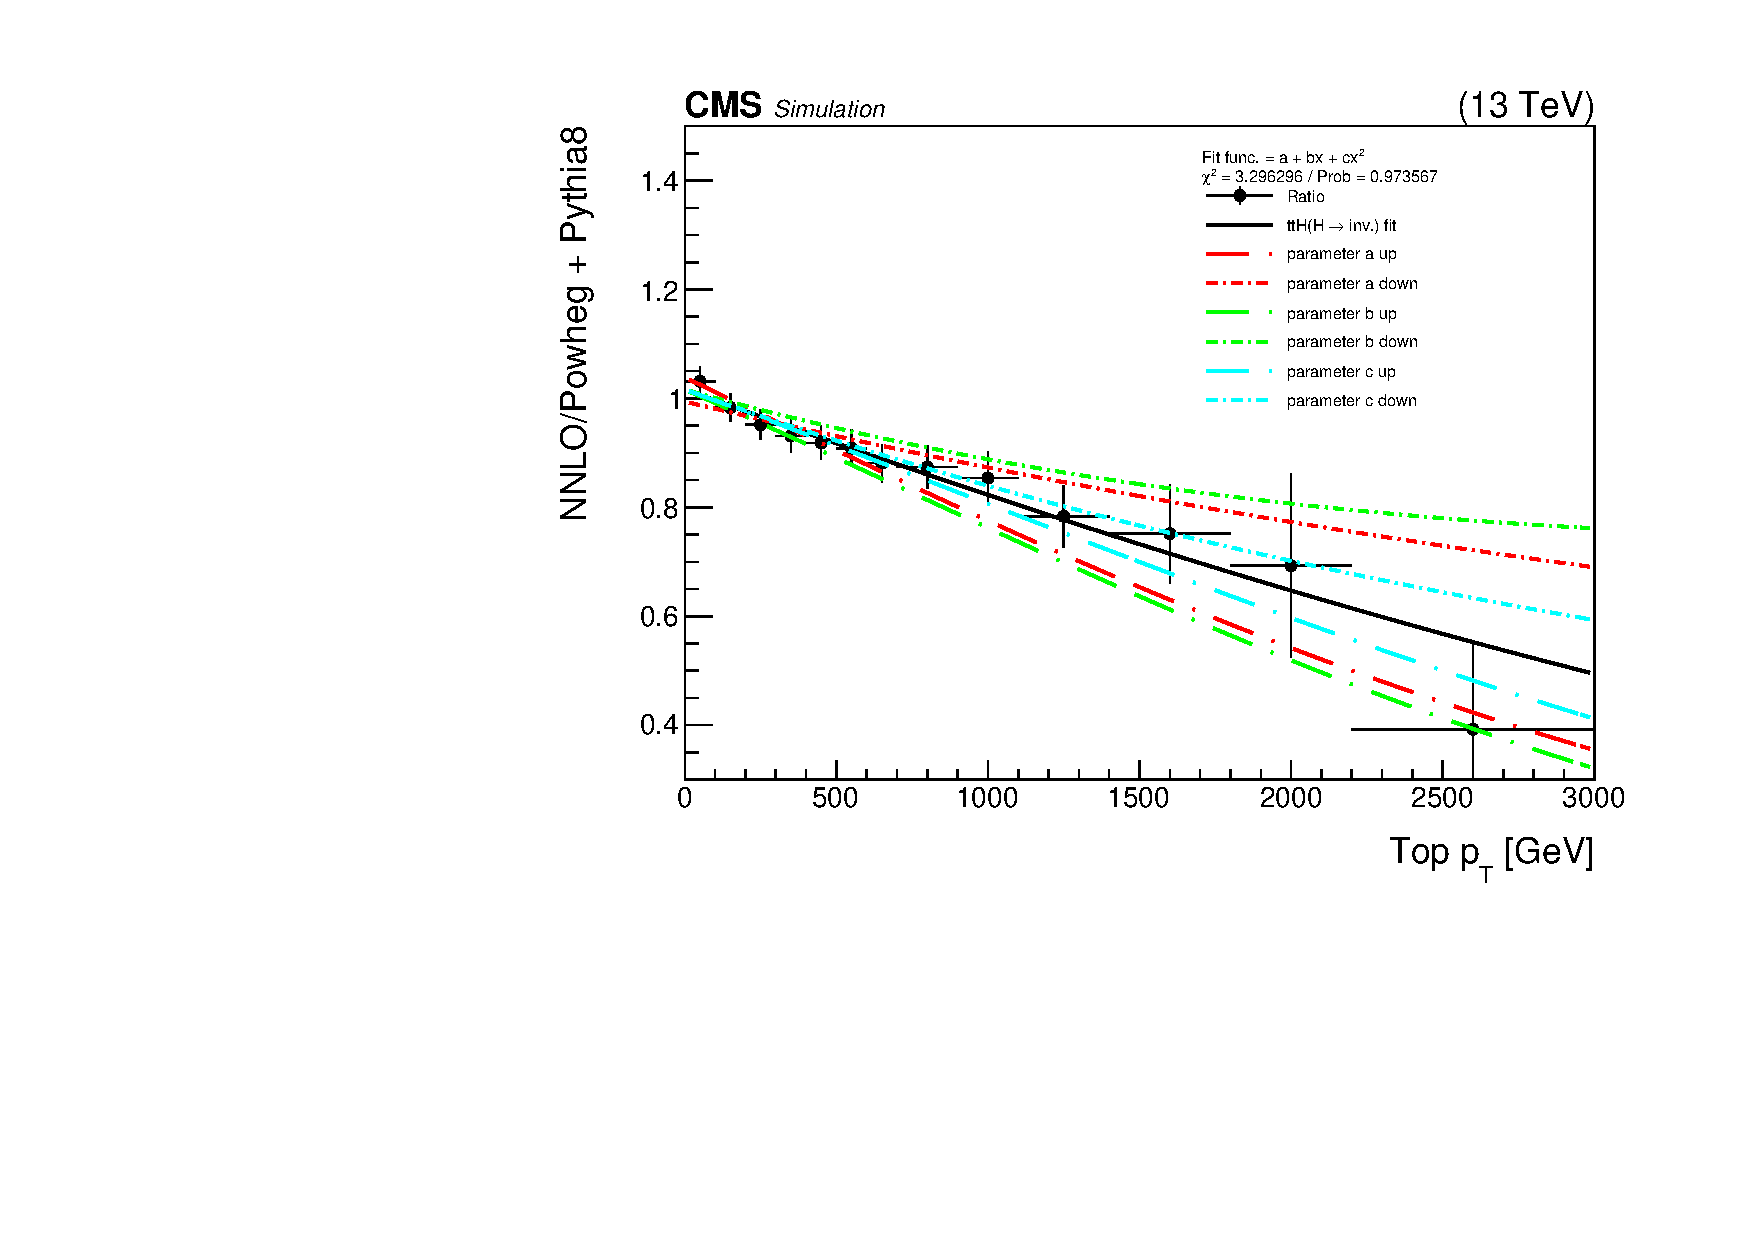
\includegraphics[width=0.6\textwidth]{figures/top_pt_reweighting/top_pt_reweighting_central.pdf}
    \caption[The ratio of the NNLO to NLO \ttbar cross section as a function of top quark \pt. The fit to the distribution---along with the uncertainties in the parameters---is shown]{The ratio of the \acrshort{nnlo} to \acrshort{nlo} \ttbar cross section as a function of top quark \pt. The fit to the distribution---along with the uncertainties in the parameters---is shown.}
    \label{fig:top_pt_reweighting}
\end{figure}

% See https://indico.cern.ch/event/904971/contributions/3857701/attachments/2036949/3410728/TopPt_20.05.12.pdf for more info


%=========================================================


\subsection{Object-level scale factors and uncertainties}
\label{subsec:htoinv_SFs_systs_objects}

There are multiple corrections applied to simulation based on the physics objects with an event as opposed to the event topology as a whole. One example of which is Sec.~\ref{subsubsec:htoinv_top_pt_reweighting}. A weight or efficiency $\epsilon$ attributed to an object itself is typically referred to as a \emph{scale factor}, while the event-level selection weight $w_{\mathrm{sel.}}$ is the efficiency for successfully tagging or selecting an event with those object contents, and is the product of the scale factors:
\begin{equation}
    w_{\mathrm{sel.}} = \prod_i^{N_\mathrm{objects}} \epsilon_i.
    \label{eq:event_selection_weight}
\end{equation}
These weights are calculated individually for each class of object in an event. For electrons, muons, and photons, these scale factors are usually from the reconstruction efficiency, identification efficiency, and \pt- or $\eta$-dependent energy corrections. In the case of \Pbottom-tagged \glspl{jet}, it is the data--simulation scale factor at the given working point from the algorithm used to identify them. Systematic uncertainties associated with the scale factors are aggregated in the same manner. Unless stated otherwise, the following scale factors and systematics are derived separately for each year in Run-2.


%=========================================================


\subsubsection{Lepton and photon identification, isolation, and reconstruction}
\label{subsubsec:htoinv_lepton_id_iso_reco_systs}

The scale factors and systematic uncertainties for electrons, photons, and muons were derived centrally for \acrshort{cms} by the \acrlong{pog}s. Electrons and photons are identified using the cut-based identification described in Secs.~\ref{subsec:objects_electrons} and \ref{subsec:objects_photons}, respectively. Scale factors are applied separately to each of these objects in simulation that account for the efficiency of identification, isolation, and reconstruction in data. They are derived as a function of $\eta$ and \acrshort{ecal} supercluster \pt. Uncertainties are given as the error in the $(\eta, \pt)$ bin of the histogram that describes the efficiencies. The ID and isolation are grouped as a single uncertainty, while reconstruction is another. Event weights simply are the products of the individual object scale factors. The uncertainty on the event weight is the product of the scale factor plus/minus its uncertainty. For each source, they are on the order of 1--5\,\%.

% While photon reconstruction efficiency is assumed to be 100\,\% for $H/E < \text{0.5}$, that is not the case for electrons. A tag and probe method is used to select electrons, distinguishing them from background objects. A gaussian is then fit to the invariant mass of the electron to capture the \PZ peak. 

% e/gamma reco SFs and systs documented here: https://twiki.cern.ch/twiki/bin/view/CMS/EgammaRunIIRecommendations#E_gamma_RECO

Muons follow a similar prescription, where the ID and isolation efficiencies are calculated in bins of $\eta$ and \pt. The systematic uncertainties for each of the two sources are separated---contrary to electrons and photons---and are usually 1\,\% or smaller in size. An equivalent reconstruction efficiency is not given as the dedicated muon chambers and reconstruction algorithms are more than sufficient.

% Muon ID/ISO info: 2016 (https://twiki.cern.ch/twiki/bin/view/CMS/MuonReferenceEffs2016LegacyRereco), 2017 (https://twiki.cern.ch/twiki/bin/view/CMS/MuonReferenceEffs2017), 2018 (https://twiki.cern.ch/twiki/bin/view/CMS/MuonReferenceEffs2018)


%=========================================================


\subsubsection{\texorpdfstring{\Pbottom-jets}{b-jets} tagged by the \texorpdfstring{\deepcsv}{DeepCSV} algorithm}
\label{subsubsec:htoinv_btagging_sfs}

Data--simulation scale factors are calculated for each \gls{bjet} as tagged by the \deepcsv algorithm. They are defined as the tagging efficiency in data divided by the efficiency for simulation for a given working point, and as a function of \gls{jet} \pt. Various methods are employed to derive separate scale factors for separate topologies, such as \acrshort{qcd} multijet or \ttbar events, and are described in Sec.~8.4 of Ref.~\citenum{Sirunyan:2017ezt}. A weighted average of the scale factors computed by each method is then taken to yield the final scale factor for a \Pbottom-tagged \gls{jet}. The resultant systematic uncertainty is typically less than 5\,\%.

% This talk goes through the methods and SFs in more detail: https://cds.cern.ch/record/2627468/files/DP2018_033.pdf


%=========================================================


\subsubsection{Boosted jets tagged by the \texorpdfstring{\deepakeight}{DeepAK8} algorithm}
\label{subsubsec:htoinv_deepak8_sfs}

In a similar fashion to the section above, objects classified by the \deepakeight algorithm are given scale factors according to the data/\acrshort{mc} efficiencies as a function of AK8 \gls{jet} \pt. Scale factors are derived separately for \glspl{jet} tagged as originating from a top quark and \PVec boson. Systematic variations associated with the scale factors on the order of 1--10\,\% are also derived separately, according to Sec.~8.1 of Ref.~\citenum{CMS-PAS-JME-18-002}.


%=========================================================


\subsection{Minor contributions}
\label{subsec:htoinv_minor_weights_systs}

In the following subsection, minor corrections and uncertainties which had little impact on the yields are documented.


%=========================================================


\subsubsection{Pre-firing in the ECAL}
\label{subsubsec:htoinv_ecal_prefiring_weight}

A weight is applied to events in simulation that emulates the effect of pre-firing in 2016 and 2017 data, given in Ref.~\citenum{prefiring_weight}:
\begin{equation}
    w_{\text{pre-firing}} = \prod_{i = \Pphoton,\, \mathrm{jet}} 1 - \epsilon_i^{\text{pre-firing}}(\eta, \pt^{\mathrm{EM}}),
    \label{eq:prefiring_weight}
\end{equation}
where $\epsilon$ is the probability for an object to pre-fire as a function of its $\eta$ and electromagnetic \pt (simply \pt for photons, and \pt multiplied by the sum of the charged and neutral electromagnetic energy fractions for \glspl{jet}). Pre-firing probabilities are assumed to be uncorrelated between photons and jets. The systematic uncertainty in the event weight is found by taking the uncertainty on $\epsilon$, defined the maximum value from either $\text{0.2}\epsilon$ or the relative statistical uncertainty in the $(\eta, \pt^{\mathrm{EM}})$ bin of the pre-firing map from which $\epsilon$ is extracted. It was found to impact the yields in the analysis by $< \text{1\,\%}$.

% Pre-firing: https://twiki.cern.ch/twiki/bin/viewauth/CMS/L1ECALPrefiringWeightRecipe, https://indico.cern.ch/event/764279/


%=========================================================


\subsubsection{Jet energy scale and resolution}
\label{subsubsec:htoinv_JES_JER_systs}

To estimate the magnitude of the \acrfull{jes} and resolution (\acrshort{jer}) uncertainties, each event is copied once per variation (i.e., upward and downward for the \acrshort{jes} and \acrshort{jer}). In the copied event, the \pt of the AK4 \glspl{jet} are varied according to scale factors from resolution/scale maps as a function of \pt and $\eta$. Consequently, the \ptvecmiss also changes for the event. The copied events are propagated through the analysis with the same treatment as the standard events. After categorisation and binning in \ptmiss, the weighted event yields from the copy in a given subcategory and \ptmiss bin serves as the uncertainty on the nominal yields.

As the event selection for the signal region is mirrored in the \glspl{CR}, variations from the \acrshort{jer} and \acrshort{jes} variations should affect both in a similar way and their effects should largely cancel in the fit to data. This cancellation is however not complete, resulting in residual differences of 2\,\% and 3\,\% on average for \acrshort{jer} and \acrshort{jes}, respectively. Similar variations for the signal processes were observed. As such, these values are applied as systematic uncertainties to all signal and background processes in all regions of the analysis.


%=========================================================


\subsubsection{Luminosity}
\label{subsubsec:htoinv_lumi_syst}

Uncertainties are associated with the various methods designed to measure the luminosity received by \acrshort{cms}. For 2016, 2017, and 2018, the total systematic uncertainties on certified data are 2.5\,\%, 2.3\,\%, and 2.5\,\%, respectively. They may be decomposed into several individual sources, some of which are correlated between years. These are documented in Tab.~\ref{tab:lumi_systs} with further information available in Refs.~\citenum{CMS-PAS-LUM-17-001}, \citenum{CMS-PAS-LUM-17-004}, and \citenum{CMS-PAS-LUM-18-002}.

\begin{table}[htbp]
    \centering
    \begin{tabular}{lccc}
        \toprule
        Uncertainty source & Impact in 2016 & Impact in 2017 & Impact in 2018 \\\midrule
        Uncorrelated sources & 2.2 & 2.0 & 1.5 \\
        $x$-$y$ factorisation & 0.9 & 0.8 & 2.0 \\
        Length scale & --- & 0.3 & 0.2 \\
        Beam-beam deflection & 0.4 & 0.4 & --- \\
        Dynamic $\beta$ & 0.5 & 0.5 & --- \\
        Beam current calibration & --- & 0.3 & 0.2 \\
        Ghosts and satellites & 0.4 & 0.1 & ---  \\
        \bottomrule
    \end{tabular}
    \caption[Sources of uncertainty in the luminosity measurements for each year of Run-2]{Sources of uncertainty in the luminosity measurements for each year of Run-2, and their impacts in percent.}
    \label{tab:lumi_systs}
\end{table}

% Lumi POG page: https://twiki.cern.ch/twiki/bin/view/CMS/TWikiLUM


%=========================================================


\subsubsection{Cross section for signal processes}
\label{subsubsec:htoinv_signal_xs_syst}

There are several sources of uncertainty in the computation of high order cross sections, from both theoretical and experimental sides. As with the nominal cross sections for signal processes, the uncertainties are retrieved from Ref.~\citenum{Cepeda:2019klc}. Each source for each signal process is treated as a separate uncertainty on the normalisation. They are correlated across years as the cross sections are constant. Nominal values of the cross sections at \comruntwo are tabulated in Tab.~\ref{tab:htoinv_signal_xsecs}. A summary of the uncertainties are presented in Tab.~\ref{tab:htoinv_signal_xs_systs}.

\begin{table}[htbp]
    \centering
    \begin{tabular}{lcc}
        \toprule
        Signal & $\delta\text{(scale)}$ (\%) & $\delta\text{(\acrshort{pdf}} + \alpha_{\mathrm{S}}\text{)}$ (\%) \\\midrule
        \ttH & $+\text{6.0}$, $-\text{9.2}$ & $\pm \text{3.5}$ \\
        \WplusH & $+\text{0.74}$, $-\text{0.73}$ & $\pm \text{1.79}$ \\
        \WminusH & $+\text{0.59}$, $-\text{0.63}$ & $\pm \text{2.03}$ \\
        $\HepProcess{\pp \to \ZH}$ & $+\text{3.50}$, $-\text{2.68}$ & $\pm \text{1.65}$ \\
        $\HepProcess{\Pgluon\Pgluon \to \ZH}$ & $+\text{2.49}$, $-\text{1.88}$ & $\pm \text{4.37}$ \\
        VBF & $+\text{0.43}$, $-\text{0.33}$ & $\pm \text{2.1}$ \\
        \bottomrule
    \end{tabular}
    \caption[Systematic uncertainties on the cross section of the simulated \higgstoinv signal samples]{Systematic uncertainties on the cross section of the simulated \higgstoinv signal samples. Values obtained from Ref.~\citenum{Cepeda:2019klc}.}
    \label{tab:htoinv_signal_xs_systs}
\end{table}


%=========================================================


\subsection{Summary of systematic uncertainties}
\label{subsec:htoinv_syst_summary}

Tab.~\ref{tab:htoinv_syst_summary} contains a summary of the systematic uncertainties incorporated in the fits to data. The type of uncertainty, whether it affects primarily the normalisation of the event yields and/or the shapes of distributions, the applicable data taking years and correlations among them, the samples affected, and estimations of the impacts on event yields on both the \ptmiss distribution and signal strength parameter $r$ are presented.

\begin{sidewaystable}[htbp]
    \small
    \centering
    \begin{tabular*}{\linewidth}{@{\extracolsep{\fill}}lccccc}
        \toprule
        Source & Type & Years & Samples & Impact on yields (\%) & Impact on $r$ (\%) \\\midrule
        Pileup & Normalisation, shape & All, correlated & All & 1--2 & $< \text{1}$ \\
        \acrshort{nlo} renormalisation scale & Normalisation, shape & All, correlated & \acrshort{lo} $\PVec \plusjets$ & 0--5 & 2 \\
        \acrshort{nlo} factorisation scale & Normalisation, shape & All, correlated & \acrshort{lo} $\PVec \plusjets$ & 1--10 & 1--2 \\
        \acrshort{nlo} \acrshort{pdf} & Normalisation, shape & All, correlated & \acrshort{lo} $\PVec \plusjets$ & 2--20 & 1--3 \\
        Trigger efficiency & Normalisation, shape & All, correlated & All & 1--2 & $< \text{1}$ \\
        QCD \muR \& \muF & Shape & All, correlated & \ttH, \ttbar, $\ttbar X$ & 0--10 & $< \text{1}$ \\
        Top \pt & Shape & All, correlated & \ttbar & $< \text{2}$ & $< \text{1}$ \\
        Muon ID & Normalisation & All, correlated & All & $< \text{1}$ & 0--4 \\
        Muon isolation & Normalisation & All, correlated & All & 1 & $< \text{1}$ \\
        Electron ID \& isolation & Normalisation & All, correlated & All & 1--5 & 1--2 \\
        Electron reconstruction & Normalisation & All, correlated & All & 1--5 & $< \text{1}$ \\
        Photon ID \& isolation & Normalisation & All, correlated & All & 1--5 & 1 \\
        Photon reconstruction & Normalisation & All, correlated & All & 1--2 & $< \text{1}$ \\
        \Pbottom-tagging with \deepcsv & Normalisation & All, correlated & All & $< \text{5}$ & 1 \\
        \deepakeight tagging & Normalisation & All, correlated & All & 1--10 & 0--5 \\
        \acrshort{ecal} pre-firing & Normalisation & 2016--17, uncorrelated & All & $< \text{1}$ & $< \text{1}$\\
        \acrlong{jer} & Normalisation & All, correlated & All & 2 & 2 \\
        \acrlong{jes} & Normalisation & All, correlated & All & 3 & 3 \\
        Luminosity & Normalisation & All & All & 2--3 & 1 \\
        Photon purity & Normalisation & All, uncorrelated & \acrshort{qcd} in \singlePhotonCr CR & 25 & $< \text{1}$ \\
        \acrshort{qcd} prediction & Normalisation & All, uncorrelated & \acrshort{qcd} in SR & 50 & 1--3 \\
        Signal cross section & Normalisation & All, correlated & Signal & 0.5--9 & $< \text{2}$ \\
        \bottomrule
    \end{tabular*}
    \caption[The experimental uncertainties present in the analysis with the applicable samples, and impacts on the corresponding event counts and overall signal strength parameter $r$]{The experimental uncertainties present in the analysis with the applicable samples (where ``all'' corresponds to all signal and background simulation), and impacts on the corresponding event counts and overall signal strength parameter $r$.}
    \label{tab:htoinv_syst_summary}
\end{sidewaystable}

\clearpage
